\chapter{Конструкторская часть}

В данном разделе производится формализация сущностей в системе, устанавливается ролевая модель и определяются необходимые процедуры, функции или триггеры. Каждой сущности, описанной в аналитической части, присваиваются соответствующие поля, содержащие информацию, необходимую для их полного определения. 

На основе этой информации разрабатывается диаграмма сущность-связь базы данных, на которой отображаются все необходимые таблицы для правильной для корректной работы приложения.

\section{Описание сущностей базы данных}

В соответствии с таблицей~\ref{tb:data}, содержащей данные, которые должны находиться в базе данных, можно выделить следующие таблицы:
\begin{enumerate}
	\item users --- таблица пользователей;
	\item zones --- таблица зон, залов, комнат антикафе;
	\item bookings --- таблица броней зон антикафе;
	\item inventories --- таблица инвентаря зон антикафе;
	\item feedbacks --- таблица отзывов пользователей о зонах антикафе;
	\item dishes --- таблица меню блюд антикафе;
	\item packages --- таблица пакетов для формирования расчета оплаты за аренду зон антикафе.
\end{enumerate}

На основе информации о выбранной СУБД и представленной на рисунке~\ref{fig:er} диаграмме сущность-связь, мы определим для каждой из указанных таблиц структуру столбцов, их типы и установим соответствующие ограничения, которые представлены на в таблицах~\ref{table:db:users}--\ref{table:db:packages}.

\begin{table}[H]
	\begin{center}
		\caption{Информация о столбцах таблицы пользователей}
		\begin{tabular}{|c|c|c|c|}
			\hline
			Столбец & Тип данных & Ограничения & Значение \\
			\hline
			id & uuid & \makecell{NOT NULL, \\ PRIMARY KEY} & \makecell{Идентификатор \\ пользователя} \\
			\hline
			last\_name & VARCHAR(64) & NOT NULL & Фамилия \\
			\hline
			first\_name & VARCHAR(64) & NOT NULL & Имя\\
			\hline
			middle\_name & VARCHAR(64) & NOT NULL & Отчество\\
			\hline
			birthday & DATE & NOT NULL & \makecell{Дата рождения}\\
			\hline
			gender & VARCHAR(64) & NOT NULL & \makecell{Пол}\\
			\hline
			email & TEXT & NOT NULL & \makecell{Электронная почта, \\ логин} \\
			\hline
			password & VARCHAR(256) & NOT NULL & \makecell{Хэш пароля} \\
			\hline
			role & VARCHAR(64) & NOT NULL & Права доступа \\
			\hline
		\end{tabular}
		\label{table:db:users}
	\end{center}
\end{table}

\begin{table}[H]
	\begin{center}
		\caption{Информация о столбцах таблицы зон антикафе}
		\begin{tabular}{|c|c|c|c|}
			\hline
			Столбец & Тип данных & Ограничения & Значение \\
			\hline
			id & uuid & \makecell{NOT NULL, \\ PRIMARY KEY} & \makecell{Идентификатор \\ зоны} \\
			\hline
			name & VARCHAR(64) & NOT NULL & Название \\
			\hline
			address & TEXT & NOT NULL & Адрес\\
			\hline
			size & NUMERIC & NOT NULL & Размер в кв. метрах\\
			\hline
		 	limit & INTEGER & NOT NULL & \makecell{Максимальное \\ количество людей \\ в зоне}\\
			\hline
			rating & NUMERIC & NOT NULL & \makecell{Рейтинг} \\
			\hline
		\end{tabular}
		\label{table:db:zones}
	\end{center}
\end{table}

\begin{table}[H]
	\begin{center}
		\caption{Информация о столбцах таблицы броней зон антикафе}
		\begin{tabular}{|c|c|c|c|}
			\hline
			Столбец & Тип данных & Ограничения & Значение \\
			\hline
			id & uuid & \makecell{NOT NULL, \\ PRIMARY KEY} & \makecell{Идентификатор \\ брони} \\
			\hline
			zone\_id &uuid & \makecell{NOT NULL, \\ FOREIGN KEY} & \makecell{Идентификатор \\ зоны} \\
			\hline
			user\_id & uuid & \makecell{NOT NULL, \\ FOREIGN KEY} & \makecell{Идентификатор \\ пользователя} \\
			\hline
			package\_id & uuid & \makecell{NOT NULL, \\ FOREIGN KEY} & \makecell{Идентификатор \\ пакета} \\
			\hline
			amount\_of\_people & INTEGER & NOT NULL & \makecell{Количество людей}\\
			\hline
			status & VARCHAR(64) & NOT NULL & \makecell{Статус}\\
			\hline
			date & DATE & NOT NULL & \makecell{Дата брони} \\
			\hline
			start\_time & TIME & NOT NULL & \makecell{Время начало \\ брони} \\
			\hline
			end\_time & TIME & NOT NULL & \makecell{Время конца \\ брони} \\
			\hline
			create\_date\_time & TIMESTAMP  & NOT NULL & \makecell{Дата и время \\ создания брони} \\
			\hline
			is\_piad & BOOLEAN  & NOT NULL & \makecell{Оплачена \\ ли бронь} \\
			\hline
			total\_price & NUMERIC  & NOT NULL & \makecell{Итоговая цена} \\
			\hline
		\end{tabular}
		\label{table:db:bookings}
	\end{center}
\end{table}

\begin{table}[H]
	\begin{center}
		\caption{Информация о столбцах таблицы инвентаря антикафе}
		\begin{tabular}{|c|c|c|c|}
			\hline
			Столбец & Тип данных & Ограничения & Значение \\
			\hline
			id & uuid & \makecell{NOT NULL, \\ PRIMARY KEY} & \makecell{Идентификатор \\ инвентаря} \\
			\hline
			zone\_id & uuid & \makecell{NOT NULL, \\ FOREIGN KEY} & \makecell{Идентификатор \\ зоны} \\
			\hline
			name & VARCHAR(64) & NOT NULL & Название \\
			\hline
			description & TEXT & NOT NULL & Описание\\
			\hline
			date\_production & DATE & NOT NULL & Дата производства\\
			\hline
			is\_written\_off & BOOLEAN & NOT NULL & \makecell{Значение \\ обозначающее \\ списан ли \\ инвентарь}\\
			\hline
		\end{tabular}
		\label{table:db:inventories}
	\end{center}
\end{table}

\begin{table}[H]
	\begin{center}
		\caption{Информация о столбцах таблицы отзывов зон антикафе}
		\begin{tabular}{|c|c|c|c|}
			\hline
			Столбец & Тип данных & Ограничения & Значение \\
			\hline
			id & uuid & \makecell{NOT NULL, \\ PRIMARY KEY} & \makecell{Идентификатор \\ отзыва} \\
			\hline
			zone\_id & uuid & \makecell{NOT NULL, \\ FOREIGN KEY} & \makecell{Идентификатор \\ зоны} \\
			\hline
			user\_id & uuid & \makecell{NOT NULL, \\ FOREIGN KEY} & \makecell{Идентификатор \\ пользователя} \\
			\hline
			date & TIMESTAMP & NOT NULL & Дата и время создания \\
			\hline
			mark & NUMERIC & NOT NULL & Оценка пользователя\\
			\hline
			message & TEXT & NOT NULL & \makecell{Комментарий пользователя}\\
			\hline
		\end{tabular}
		\label{table:db:feedbacks}
	\end{center}
\end{table}

\begin{table}[H]
	\begin{center}
		\caption{Информация о столбцах таблицы меню блюд антикафе}
		\begin{tabular}{|c|c|c|c|}
			\hline
			Столбец & Тип данных & Ограничения & Значение \\
			\hline
			id & uuid & \makecell{NOT NULL, \\ PRIMARY KEY} & \makecell{Идентификатор \\ блюда} \\
			\hline
			name & VARCHAR(64) & NOT NULL & Название \\
			\hline
			type & VARCHAR(64) & NOT NULL & \makecell{Тип блюда} \\
			\hline
			price & NUMERIC & NOT NULL & Цена в рублях \\
			\hline
			description & TEXT & NOT NULL & Описание \\
			\hline
		\end{tabular}
		\label{table:db:dishes}
	\end{center}
\end{table}

\begin{table}[H]
	\begin{center}
		\caption{Информация о столбцах таблицы пакетов антикафе}
		\begin{tabular}{|c|c|c|c|}
			\hline
			Столбец & Тип данных & Ограничения & Значение \\
			\hline
			id & uuid & \makecell{NOT NULL, \\ PRIMARY KEY} & \makecell{Идентификатор \\ пакета} \\
			\hline
			name & VARCHAR(64) & NOT NULL & Название \\
			\hline
			type & VARCHAR(64) & NOT NULL & \makecell{Тип пакета} \\
			\hline
			price & NUMERIC & NOT NULL & Цена в рублях \\
			\hline
			rental\_time & INTEGER & NOT NULL & \makecell{Количество времени \\ проведения} \\
			\hline
			description & TEXT & NOT NULL & Описание \\
			\hline
		\end{tabular}
		\label{table:db:packages}
	\end{center}
\end{table}

\clearpage

На рисунке~\ref{fig:db} приведена ER-диаграмма базы данных.
\begin{figure}[h]
	\centering
	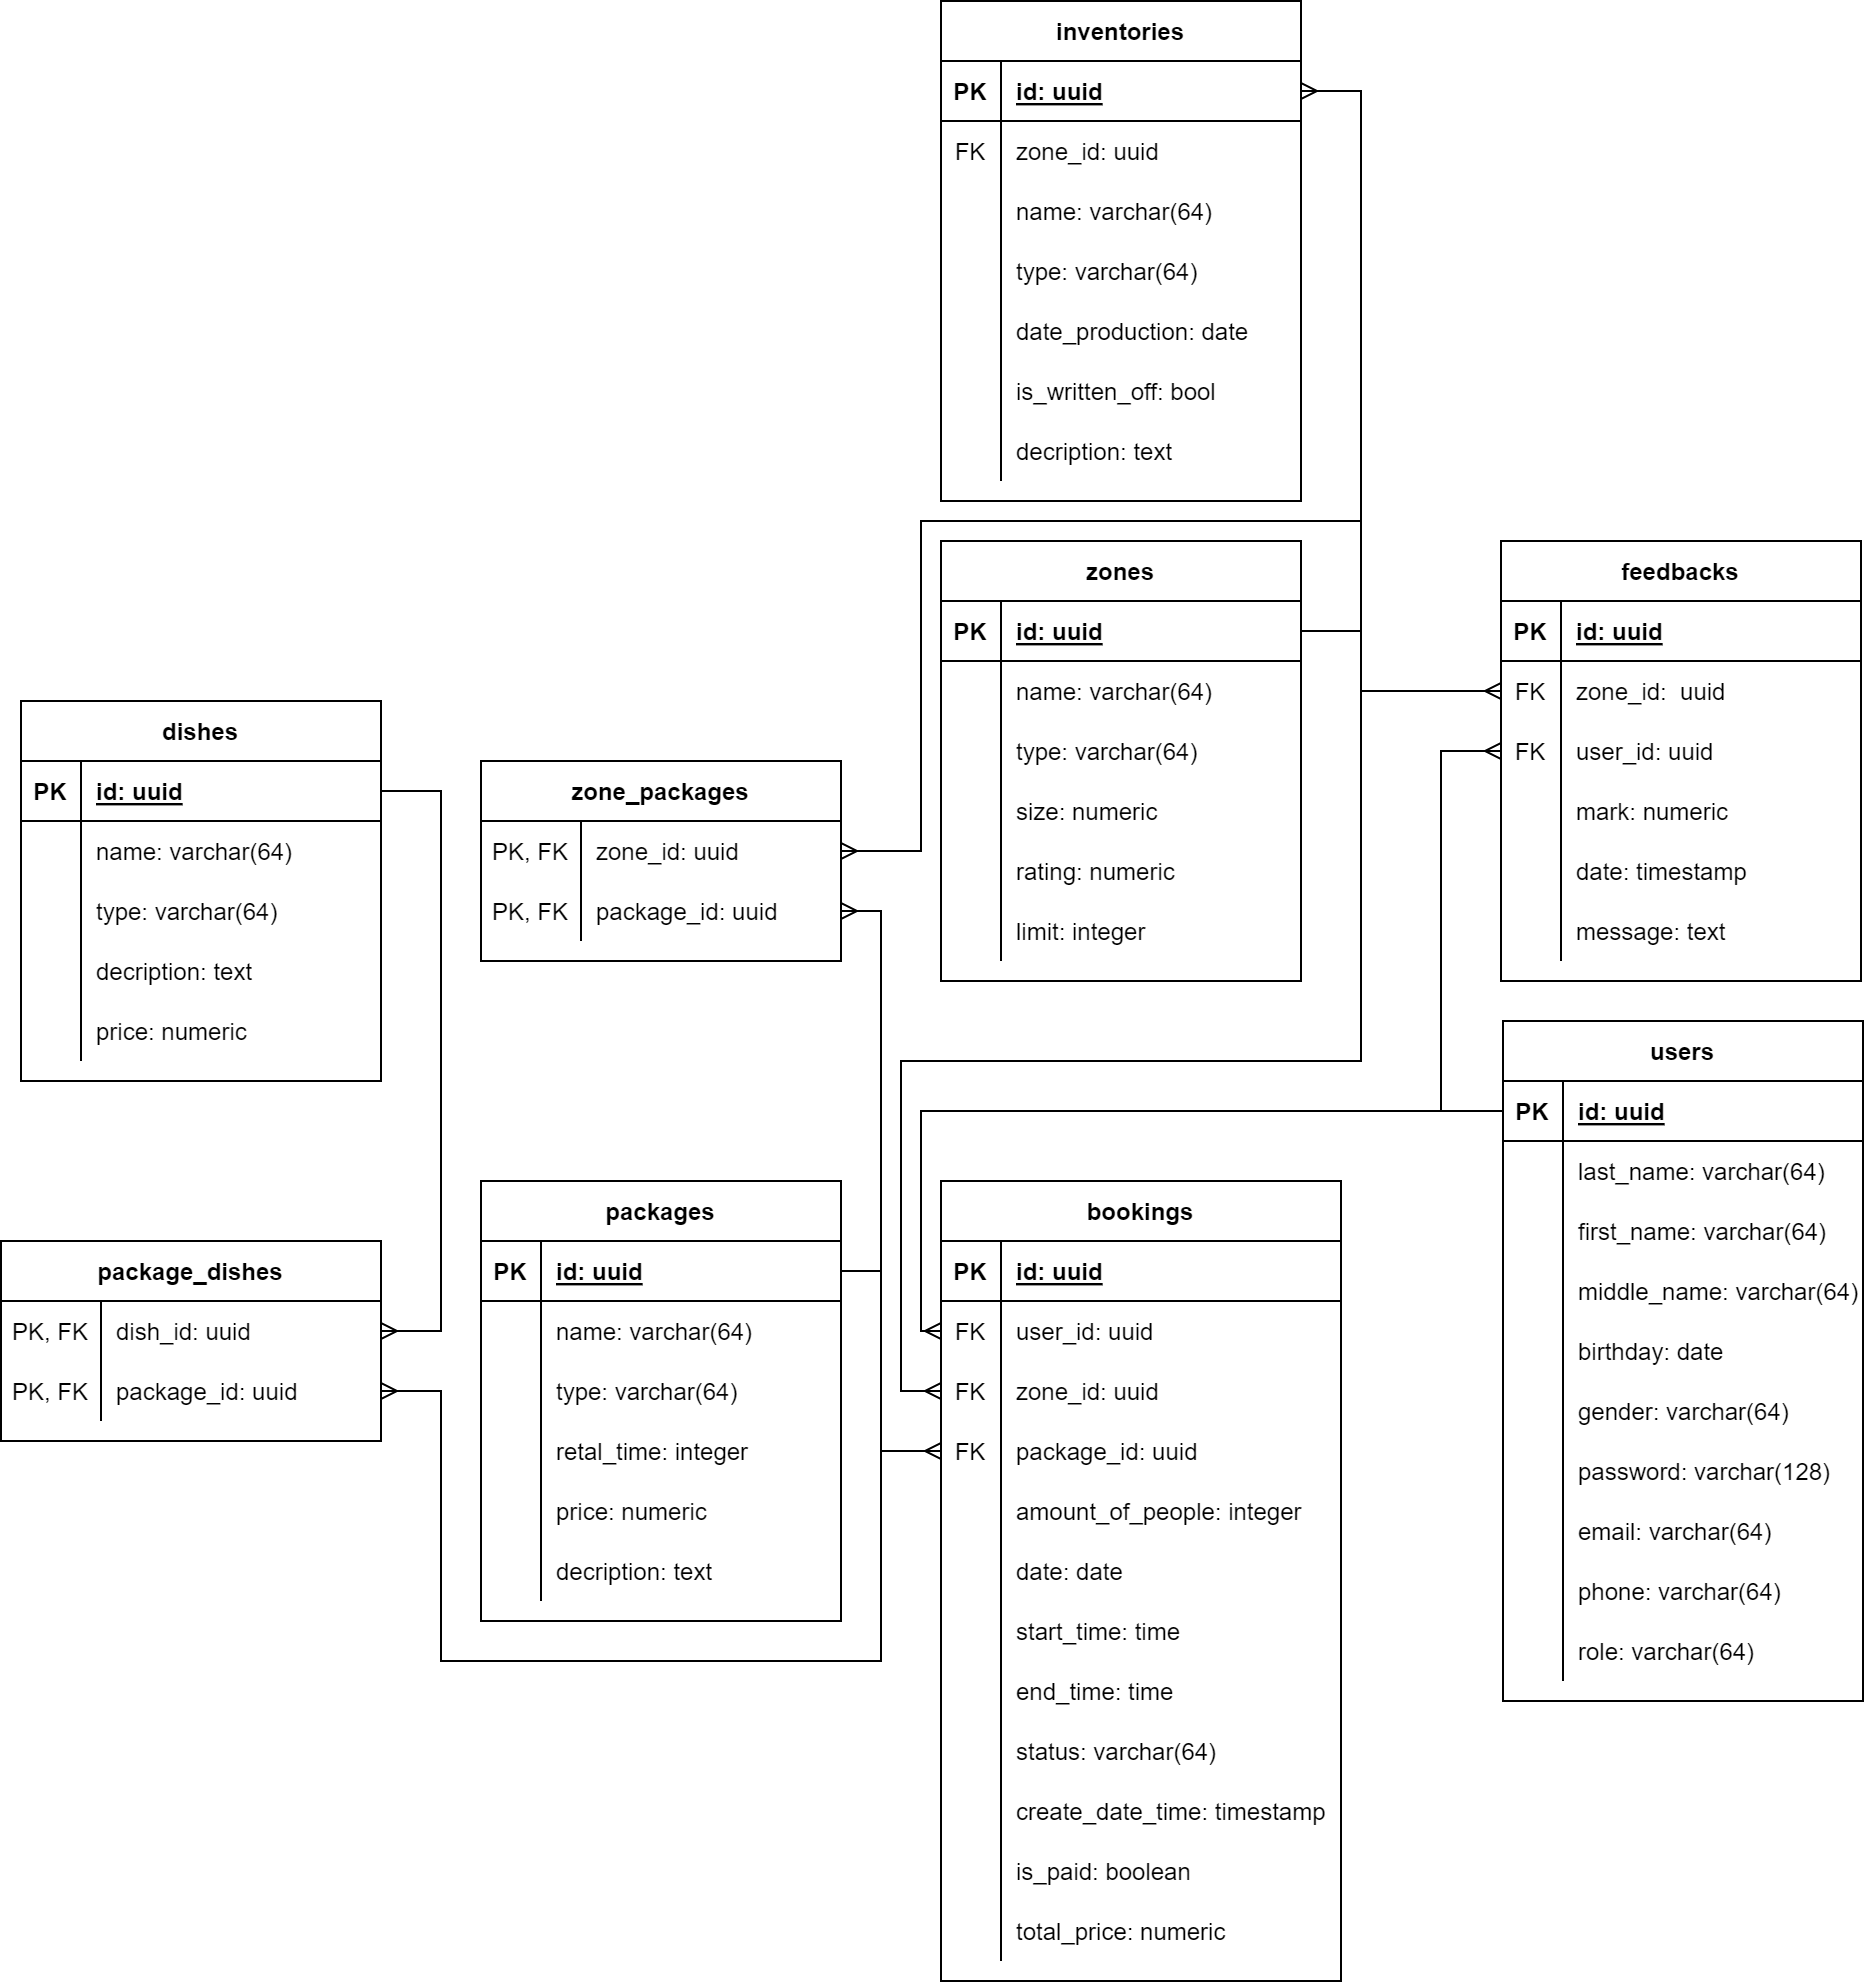
\includegraphics[width=0.9\textwidth]{img/db-diagram.png}
	\caption{ER-диаграмма базы данных}
	\label{fig:db}
\end{figure}

\section{Ролевая модель}

Ролевая модель в системе играет важную роль в организации работы пользователей, обеспечивая им доступ к определенному набору функций в системе.

Что касается работы пользователей с базой данных, то для этой цели определена следующая ролевая модель:

\begin{itemize}
	\item Гость имеет права доступ SELECT ко всем таблицам, кроме таблиц пользователей и броней, INSERT только к таблице пользователей;
	\item Авторизованный пользователь имеет права доступа SELECT ко всем таблицам, INSERT только к таблице броней, UPDATE к таблицам броней и пользователей;
	\item Администратор имеет все права доступа ко всем таблицам.
\end{itemize}

\section{Используемые триггеры}

В базе данных будет присутствовать специальный триггер, который активируется автоматически после добавления новой записи в таблицу отзывов. Этот триггер выполняет пересчет рейтинга соответствующей зоны антикафе на основе оценки, указанной в отзыве пользователем. При каждой вставке новых данных в таблицу отзывов, данный триггер будет автоматически вызываться, обеспечивая актуальность рейтинга.

\clearpage

На рисунке~\ref{trigger:calcrating} представлена схема триггера.

\begin{figure}[h]
	\centering
	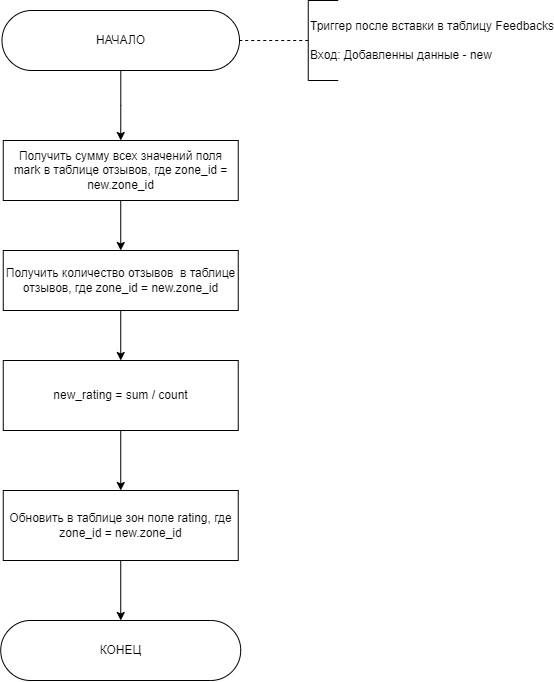
\includegraphics[width=0.65\textwidth]{img/calc-rating.png}
	\caption{Схема алгоритма триггера после добавления записи в таблицу feedbacks}
	\label{trigger:calcrating}
\end{figure}

\section{Диаграмма классов приложения}

Приложение строится согласно диаграмме классов, приведенной на рисунке~\ref{fig:appclass}.
На диаграмме классов представлена схема реализаций как части доступа базы данных, то есть реализация паттерна <<Репозитория>> для каждой сущности базы данных и части бизнес логики, где реализованы сервисы по обработки данных в необходимый вид для пользователя.

\clearpage

\begin{figure}[h]
	\centering
	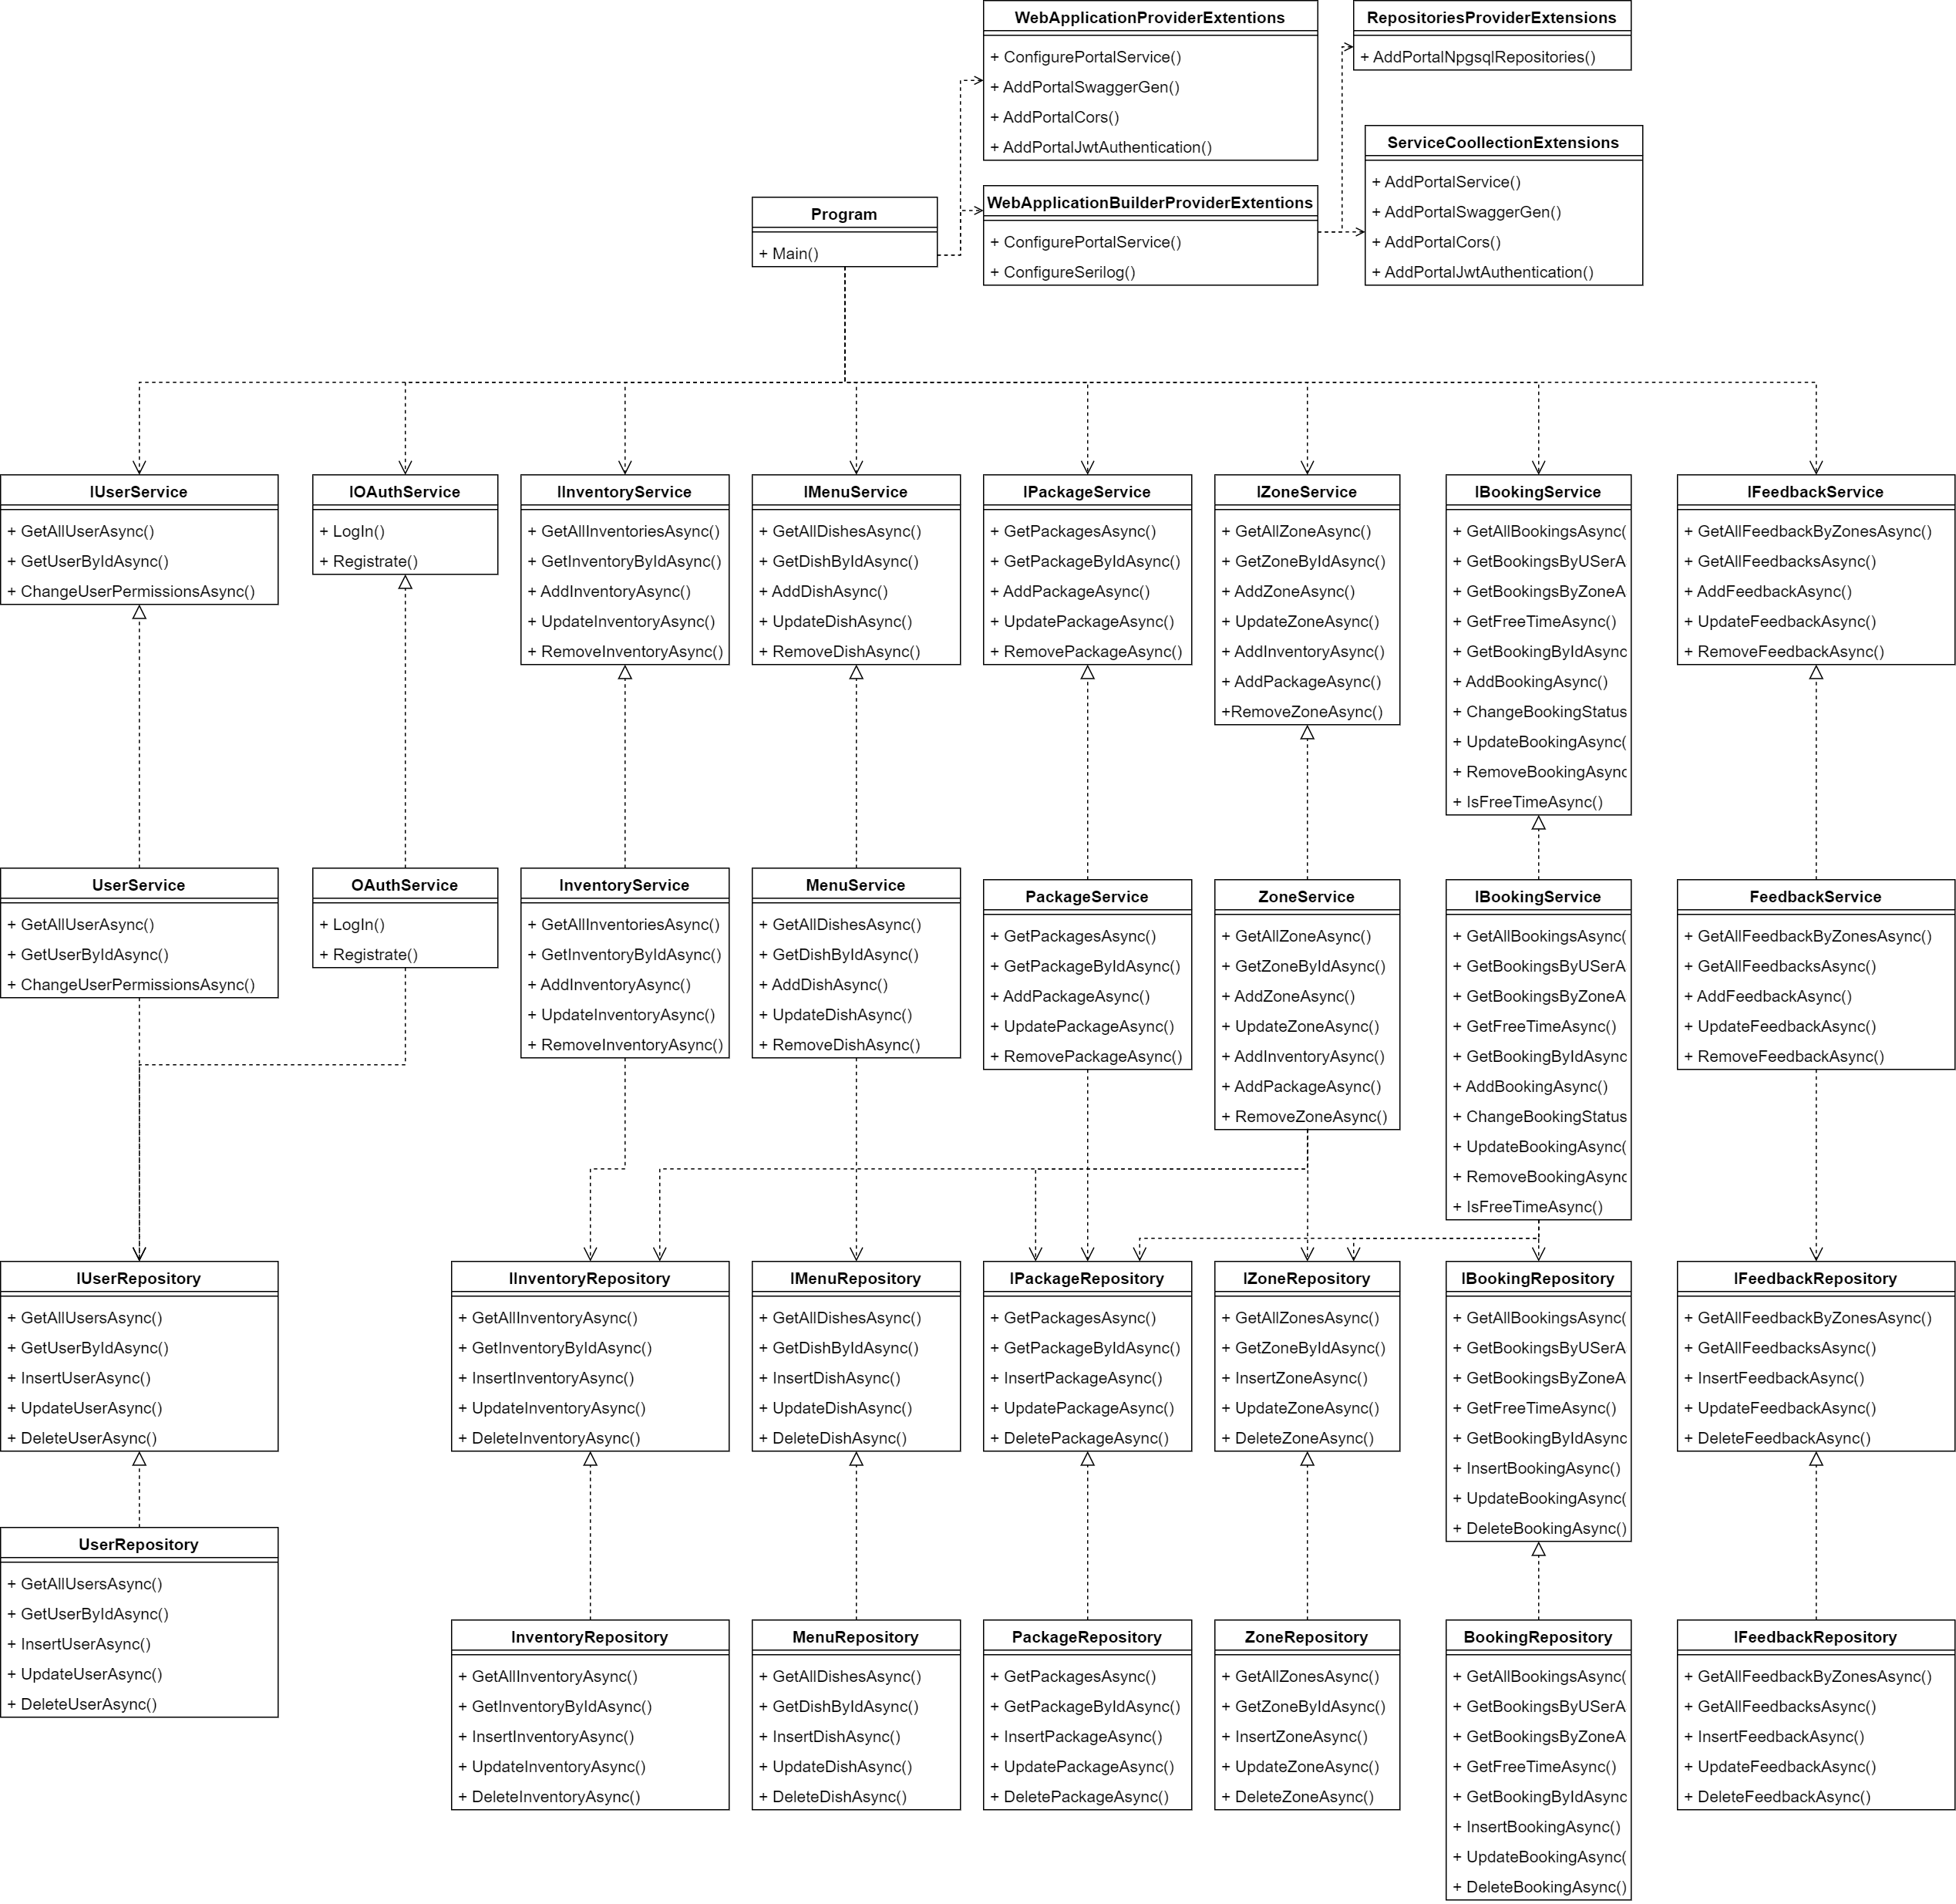
\includegraphics[width=0.9\textwidth]{img/app-class.png}
	\caption{Диаграмма классов приложения}
	\label{fig:appclass}
\end{figure}

\section*{Вывод}

В данном разделе были описаны все сущности базы данных на основе анализа предметной области, представлена ER-диаграмма сущностей, описана ролевая модель.
Также был спроектирован необходимые триггеры, функции или процедуры. 
Приведена диаграмма классов приложения, которое будет разработана для интеграции с базой данных.